\documentclass[dvipdfmx,11pt,a4paper]{jsarticle}
\usepackage{amsmath,amssymb}
\usepackage{amsthm}
\usepackage{ascmac}
\usepackage{bm}
\usepackage[dvipdfmx]{graphicx}	% required for `\includegraphics' (yatex added)
\usepackage{setspace}           % required for `\doublespace'
\usepackage{tikz}
\usepackage{tikz-cd}
\usetikzlibrary{angles, positioning, shapes, arrows.meta, decorations.pathmorphing}
%\usetikzlibrary{intersections, calc, arrows, positioning, arrows.meta}
\usepackage{tcolorbox}  % 定理環境の装飾
\tcbuselibrary{skins, breakable, theorems}
\usepackage{xcolor}
\usepackage{natbib}
\usepackage{pxrubrica}
\usepackage[margin=30truemm, left=40truemm, right=40truemm]{geometry}
\usepackage{thmbox}     % required for theorem environment with side bar
%
\setlength{\parskip}{3mm} %段落間にスペースを入れる


% \pagestyle{myheadings}
% \markright{\footnotesize \sf 2022秋期「哲学者のための数学」授業資料(大塚淳) \ \ 配布禁止}


\theoremstyle{definition}
\newtheorem[S]{exercise}{練習問題}[section]
\newtheorem[S]{example}{事例}[section]
\newtheorem[S]{fact}{事実}[section]
\newtheorem[S]{attn}{注意}[section]
\newtheorem[S]{develop}{発展}[section]
\renewcommand{\theattn}{}

\newtcbtheorem[auto counter, number within=section]{rei}{事例}{
    breakable,
    coltitle=black,
    fonttitle=\bfseries,
    enhanced, colback=white, frame hidden, borderline west = {0.5pt}{5pt}{black},
%    number freestyle={\noexpand\thesection.\noexpand\arabic{\tcbcounter}}
}{rei}

\newtcbtheorem[auto counter, number within=section]{prop}{命題}{
    breakable,
    coltitle=black,
    fonttitle=\bfseries,
    enhanced, colback=white, frame hidden, borderline west = {0.5pt}{5pt}{black},
%    number freestyle={\noexpand\thesection.\noexpand\arabic{\tcbcounter}}
}{prop}

\newtcbtheorem[number within=section]{renshu}{練習問題}{
    breakable,
    coltitle=black,
    fonttitle=\bfseries,
    enhanced, colback=white, frame hidden, borderline west = {0.5pt}{5pt}{black}
}{renshu}


\newtcbtheorem[number within=section]{hatten}{発展}{
    breakable,
    coltitle=black,
    fonttitle=\bfseries,
    enhanced, colback=white, frame hidden, borderline west = {0.5pt}{5pt}{black}
}{renshu}


\newtcbtheorem[number within=section]{dfn}{定義}{
    fonttitle=\bfseries,
    enhanced, colback=white
}{dfn}


% Bold face capital letters:
\newcommand{\bfzero}{\boldsymbol{0}}
\newcommand{\bfone}{\boldsymbol{1}}
\newcommand{\bfA}{\boldsymbol{A}}
\newcommand{\bfB}{\boldsymbol{B}}
\newcommand{\bfC}{\boldsymbol{C}}
\newcommand{\bfD}{\boldsymbol{D}}
\newcommand{\bfE}{\boldsymbol{E}}
\newcommand{\bfF}{\boldsymbol{F}}
\newcommand{\bfG}{\boldsymbol{G}}
\newcommand{\bfH}{\boldsymbol{H}}
\newcommand{\bfI}{\boldsymbol{I}}
\newcommand{\bfJ}{\boldsymbol{J}}
\newcommand{\bfK}{\boldsymbol{K}}
\newcommand{\bfL}{\boldsymbol{L}}
\newcommand{\bfM}{\boldsymbol{M}}
\newcommand{\bfN}{\boldsymbol{N}}
\newcommand{\bfO}{\boldsymbol{O}}
\newcommand{\bfP}{\boldsymbol{P}}
\newcommand{\bfQ}{\boldsymbol{Q}}
\newcommand{\bfR}{\boldsymbol{R}}
\newcommand{\bfS}{\boldsymbol{S}}
\newcommand{\bfT}{\boldsymbol{T}}
\newcommand{\bfU}{\boldsymbol{U}}
\newcommand{\bfV}{\boldsymbol{V}}
\newcommand{\bfW}{\boldsymbol{W}}
\newcommand{\bfX}{\boldsymbol{X}}
\newcommand{\bfY}{\boldsymbol{Y}}
\newcommand{\bfZ}{\boldsymbol{Z}}

\newcommand{\bfa}{\boldsymbol{a}}
\newcommand{\bfb}{\boldsymbol{b}}
\newcommand{\bfc}{\boldsymbol{c}}
\newcommand{\bfd}{\boldsymbol{d}}
\newcommand{\bfe}{\boldsymbol{e}}
\newcommand{\bff}{\boldsymbol{f}}
\newcommand{\bfk}{\boldsymbol{k}}
\newcommand{\bfm}{\boldsymbol{m}}
\newcommand{\bfn}{\boldsymbol{n}}
\newcommand{\bfo}{\boldsymbol{o}}
\newcommand{\bfp}{\boldsymbol{p}}
\newcommand{\bfq}{\boldsymbol{q}}
\newcommand{\bfr}{\boldsymbol{r}}
\newcommand{\bfs}{\boldsymbol{s}}
\newcommand{\bft}{\boldsymbol{t}}
\newcommand{\bfu}{\boldsymbol{u}}
\newcommand{\bfv}{\boldsymbol{v}}
\newcommand{\bfw}{\boldsymbol{w}}
\newcommand{\bfx}{\boldsymbol{x}}
\newcommand{\bfy}{\boldsymbol{y}}
\newcommand{\bfz}{\boldsymbol{z}}



% BB (???) capital letters:
\newcommand{\bbA}{\mathbb{A}}
\newcommand{\bbB}{\mathbb{B}}
\newcommand{\bbC}{\mathbb{C}}
\newcommand{\bbD}{\mathbb{D}}
\newcommand{\bbE}{\mathbb{E}}
\newcommand{\bbF}{\mathbb{F}}
\newcommand{\bbG}{\mathbb{G}}
\newcommand{\bbI}{\mathbb{I}}
\newcommand{\bbN}{\mathbb{N}}
\newcommand{\bbP}{\mathbb{P}}
\newcommand{\bbQ}{\mathbb{Q}}
\newcommand{\bbR}{\mathbb{R}}
\newcommand{\bbU}{\mathbb{U}}
\newcommand{\bbV}{\mathbb{V}}
\newcommand{\bbX}{\mathbb{X}}
\newcommand{\bbY}{\mathbb{Y}}
\newcommand{\bbZ}{\mathbb{Z}}
\newcommand{\bbone}{{\ifmmode\mathrm{1\!l}\else\mbox{\(\mathrm{1\!l}\)}\fi}}


% Caligraphic math capital letters:
\newcommand{\mcalA}{\mathcal{A}}
\newcommand{\mcalB}{\mathcal{B}}
\newcommand{\mcalC}{\mathcal{C}}
\newcommand{\mcalD}{\mathcal{D}}
\newcommand{\mcalE}{\mathcal{E}}
\newcommand{\mcalF}{\mathcal{F}}
\newcommand{\mcalG}{\mathcal{G}}
\newcommand{\mcalH}{\mathcal{H}}
\newcommand{\mcalI}{\mathcal{I}}
\newcommand{\mcalJ}{\mathcal{J}}
\newcommand{\mcalK}{\mathcal{K}}
\newcommand{\mcalL}{\mathcal{L}}
\newcommand{\mcalM}{\mathcal{M}}
\newcommand{\mcalN}{\mathcal{N}}
\newcommand{\mcalO}{\mathcal{O}}
\newcommand{\mcalP}{\mathcal{P}}
\newcommand{\mcalQ}{\mathcal{Q}}
\newcommand{\mcalS}{\mathcal{S}}
\newcommand{\mcalT}{\mathcal{T}}
\newcommand{\mcalU}{\mathcal{U}}
\newcommand{\mcalV}{\mathcal{V}}
\newcommand{\mcalX}{\mathcal{X}}
\newcommand{\mcalY}{\mathcal{Y}}
\newcommand{\mcalZ}{\mathcal{Z}}

% Graph nodes notations:
\newcommand{\PA}{\mathit{PA}}
\newcommand{\bfPA}{\mathbf{PA}}
\newcommand{\CH}{\mathit{CH}}
\newcommand{\bfCH}{\mathbf{CH}}
\newcommand{\DS}{\mathit{DS}}
\newcommand{\bfDS}{\mathbf{DS}}
\newcommand{\ND}{\mathit{ND}}
\newcommand{\bfND}{\mathbf{ND}}
\newcommand{\AN}{\mathit{an}}
\newcommand{\bfAN}{\mathbf{an}}
\newcommand{\pa}{\mathit{pa}}
\newcommand{\bfpa}{\mathbf{pa}}
\newcommand{\ch}{\mathit{ch}}
\newcommand{\bfch}{\mathbf{ch}}
\newcommand{\ds}{\mathit{ds}}
\newcommand{\bfds}{\mathbf{ds}}
\newcommand{\nd}{\mathit{nd}}
\newcommand{\bfnd}{\mathbf{nd}}
\newcommand{\an}{\mathit{an}}
\newcommand{\bfan}{\mathbf{an}}



\DeclareMathOperator*{\argmax}{arg\,max}
\DeclareMathOperator*{\argmin}{arg\,min}
\DeclareMathOperator*{\argsup}{arg\,sup}
\DeclareMathOperator*{\arginf}{arg\,inf}
\DeclareMathOperator{\erfc}{erfc}
\DeclareMathOperator{\diag}{diag}
\DeclareMathOperator{\cum}{cum}
\DeclareMathOperator{\sgn}{sgn}
\DeclareMathOperator{\tr}{tr}
\DeclareMathOperator{\spn}{span}
\DeclareMathOperator{\adj}{adj}
\DeclareMathOperator{\E}{\mathbb{E}}
\DeclareMathOperator{\var}{Var}
\DeclareMathOperator{\cov}{Cov}
\DeclareMathOperator{\corr}{corr}
\DeclareMathOperator{\sech}{sech}
\DeclareMathOperator{\sinc}{sinc}
\DeclareMathOperator*{\lms}{l.i.m.\,}
\newcommand{\varop}[1]{\var\left[{#1}\right]}
\newcommand{\covop}[2]{\cov\left({#1},{#2}\right)}
\newcommand{\T}{^\textrm{T}}
\newcommand\indep{\protect\mathpalette{\protect\independenT}{\perp}}
\def\independenT#1#2{\mathrel{\rlap{$#1#2$}\mkern2mu{#1#2}}}

\newcommand{\bfalpha}{\boldsymbol{\alpha}}
\newcommand{\bfbeta} {\boldsymbol{\beta}}
\newcommand{\bfgamma}{\boldsymbol{\gamma}}
\newcommand{\bfeta}  {\boldsymbol{\eta}}
\newcommand{\bftheta}{\boldsymbol{\theta}}
\newcommand{\bflambda}   {\boldsymbol{\lambda}}
\newcommand{\bfmu}   {\boldsymbol{\mu}}
\newcommand{\bfnu}   {\boldsymbol{\nu}}
\newcommand{\bfxi}   {\boldsymbol{\xi}}
\newcommand{\bfpsi}  {\boldsymbol{\psi}}
\newcommand{\bfphi}   {\boldsymbol{\phi}}
\newcommand{\bfrho}   {\boldsymbol{\rho}}
\newcommand{\bfvarepsilon}{\boldsymbol{\varepsilon}}
%\newcommand{\qed}{{qed}}
%\newcommand{\eqalignno}[1]{\begin{array}{ccccccc}#1\end{array}}

\newcommand{\bfGamma}{\boldsymbol{\Gamma}}
\newcommand{\bfTheta}{\boldsymbol{\Theta}}
\newcommand{\bfLambda}   {\boldsymbol{\Lambda}}
\newcommand{\bfPsi}  {\boldsymbol{\Psi}}
\newcommand{\bfPhi}   {\boldsymbol{\Phi}}
\newcommand{\bfSigma}  {\boldsymbol{\Sigma}}
\newcommand{\bfOmega}  {\boldsymbol{\Omega}}


% DISTRIBUTIOoNS: 
\newcommand{\normal}{\mathcal{N}}
\newcommand{\binomial}{\mathcal{B}}
\newcommand{\multinomial}{\mathcal{M}}
\newcommand{\exponential}{\mathcal{E}}
\newcommand{\geometric}{\mathcal{G}}
\newcommand{\poisson}{\mbox{Poisson}}
\newcommand{\uniform}{\mbox{Uniform}}

% Logic
\newcommand{\true}{\texttt{true}}
\newcommand{\false}{\texttt{false}}


%PSTricks (commande for latent nodes)
\newcommand{\lnode}[4]{ \cnode(#1){#2}{#3}\rput(#1){\footnotesize#4} }

% KEEPING TRACK OF WORK
\newcommand{\todo}[1]
{
{\color{red}{
[TODO: #1]}}
\addcontentsline{toc}{subsection}{TO DO: #1}
}

\newcommand{\fixme}[1]{{\color{red}{#1}}}

\newenvironment{answer}[1]
{\par \color{blue}{#1}}
{}


\newcommand{\note}[2]
{
{\color{red}{
[#1: #2]}}
}




\makeatletter
% define \citepos for posesive citation (e.g. Otsuka's (2015))
\DeclareRobustCommand\citepos
  {\begingroup
   \let\NAT@nmfmt\NAT@posfmt% ...except with a different name format
   \NAT@swafalse\let\NAT@ctype\z@\NAT@partrue
   \@ifstar{\NAT@fulltrue\NAT@citetp}{\NAT@fullfalse\NAT@citetp}}

\let\NAT@orig@nmfmt\NAT@nmfmt
\def\NAT@posfmt#1{\NAT@orig@nmfmt{#1's}}
\makeatother




% Code for drawing color circle used in topology (pathconnectedness)
\usepackage{xparse}
\ExplSyntaxOn

\keys_define:nn { colour_transition_circle } {
    inner   .fp_set:N   = \l__inner_radius,
    inner   .initial:n  = {2},
    outer   .fp_set:N   = \l__outer_radius,
    outer   .initial:n  = {3},
    angle   .fp_set:N   = \l__start_angle,
    angle   .initial:n  = {0}
}

\NewDocumentCommand \ColourTransitionCircle { O{} m } {
\group_begin:
    \keys_set:nn { colour_transition_circle } {#1}
    \clist_clear:N \l_tmpa_clist
    \clist_map_inline:nn {#2} {
        \clist_put_right:Nn \l_tmpa_clist {##1}
        %\clist_put_right:Nn \l_tmpa_clist {##1}
    }
    \exp_args:Nx \col_trans_circ:n \l_tmpa_clist
\group_end:
}

\cs_new_protected:Npn \col_trans_circ:n #1 {
    \int_step_inline:nnnn {1} {1} {\clist_count:n {#1} - 1} {
        \path[top~color=\clist_item:nn {#1} {##1}, bottom~color=\clist_item:nn {#1} {##1+1}, shading~angle={270-(180-360/\clist_count:n {#1})/2+(##1-1)*360/\clist_count:n {#1}+\fp_use:N \l__start_angle}] ({\fp_use:N \l__inner_radius*cos((##1-1)*360/\clist_count:n {#1}+\fp_use:N \l__start_angle)},{\fp_use:N \l__inner_radius*sin((##1-1)*360/\clist_count:n {#1}+\fp_use:N \l__start_angle)}) arc[radius = \fp_use:N \l__inner_radius, start~angle={(##1-1)*360/\clist_count:n {#1}+\fp_use:N \l__start_angle}, delta~angle=360/\clist_count:n {#1}] -- ({\fp_use:N \l__outer_radius*cos(##1*360/\clist_count:n {#1}+\fp_use:N \l__start_angle)},{\fp_use:N \l__outer_radius*sin(##1*360/\clist_count:n {#1}+\fp_use:N \l__start_angle)}) arc[radius = \fp_use:N \l__outer_radius, start~angle={##1*360/\clist_count:n {#1}+\fp_use:N \l__start_angle}, delta~angle=-360/\clist_count:n {#1}] -- cycle;
    }
    \path[top~color=\clist_item:nn {#1} {\clist_count:n {#1}}, bottom~color=\clist_item:nn {#1} {1}, shading~angle={180-180/\clist_count:n {#1}+\fp_use:N \l__start_angle}]({\fp_use:N \l__inner_radius*cos((\clist_count:n {#1}-1)*360/\clist_count:n {#1}+\fp_use:N \l__start_angle)},{\fp_use:N \l__inner_radius*sin((\clist_count:n {#1}-1)*360/\clist_count:n {#1}+\fp_use:N \l__start_angle)}) arc[radius = \fp_use:N \l__inner_radius, start~angle={(\clist_count:n {#1}-1)*360/\clist_count:n {#1}+\fp_use:N \l__start_angle}, delta~angle=360/\clist_count:n {#1}] -- ({\fp_use:N \l__outer_radius*cos(\clist_count:n {#1}*360/\clist_count:n {#1}+\fp_use:N \l__start_angle)},{\fp_use:N \l__outer_radius*sin(\clist_count:n {#1}*360/\clist_count:n {#1}+\fp_use:N \l__start_angle)}) arc[radius = \fp_use:N \l__outer_radius, start~angle={\clist_count:n {#1}*360/\clist_count:n {#1}+\fp_use:N \l__start_angle}, delta~angle=-360/\clist_count:n {#1}] -- cycle;
}

\ExplSyntaxOff
\begin{document}


\title{3. 順序}
\author{2023秋期「哲学者のための数学」授業資料(大塚淳)}
\date{ver. \today}
\maketitle

\section{構造}
前章までで,集合論の(ほんの)基礎的なところを見た.
現代数学において,集合はあらゆる理論的構造の「素材」としての役割を担っている.
例えば線形代数や解析学やリー代数や確率論や・・・あらゆる数学理論は,「かくかくしかじかの性質を持った集合」と定義できるのである\footnote{こうした集合論に根ざした数学の統一的理解は,20世紀のニコラ・ブルバキ(Nicolas Bourbaki)の仕事に多くを負っている.ブルバキは集合論をいわば数学の共通言語に見立て,各数学理論を集合論の枠内で再構築した.ちなみにブルバキはペンネームで,実際は複数の数学者の集まり(集合!)である.}.
つまり語弊を恐れずにいえば,数学の理論とは,何らかの構造を持った集合である.
実際,この章以下で我々は,ブール代数や群,位相などを,特定の構造を持つ集合として導入する.
集合が持つそうした構造は,一般に\emph{公理}(axioms)の形で表される.
まず手始めに,一番簡単な,順序構造を集合に入れるところから考えてみよう.


\section{さまざまな順序}
順序とは,特殊な条件(公理)を満たす2項関係である.
その条件の付け加え方によって,前順序/半順序/全順序という三つの順序が得られる.
以下見るように,後の方ほどより要件が多く,より「厳しい」順序になってくる.


\subsection{前順序}
同値類とは反射的,対称的かつ推移的な関係だったことを思い出そう(2章3節).
この条件から対称性を落とすと,0章でも見た\emph{前順序}ないし\emph{擬順序}(preorder)が得られる.
きちんと定義すると以下のようになる.

\begin{dfn}{前順序}{}
集合$X$上の2項関係$\preceq$が,すべての$x, y, z\in X$について以下を満たすとき,\emph{前順序}ないし\emph{擬順序}といわれる.
\begin{itemize}
 \item[O1] 反射性:$x \preceq x$
 \item[O2] 推移性:$x \preceq y$かつ$y \preceq z$ならば$x \preceq z$
% \item 反対称性:$x \preceq y$かつ$y \preceq x$ならば$x = y$
\end{itemize}
また組$\langle X, \preceq \rangle$を,\emph{前順序集合}という. 
\end{dfn}
%また集合$X$とその上に定義された前順序関係$\preceq$の組$\langle X, \preceq \rangle$を,\emph{前順序集合}という.

これは我々が今後多数見ていくことになる数学的構造の最初の例である.
一般に数学的構造は,元となる集合(この場合$X$)と,その上に定義された関係や演算からなる.
そして公理は,それがどのような関係・演算かを定めることによって,数学的構造を特徴づける.
ここでは反射性(O1)と推移性(O2)という2つの公理が,関係$\preceq$および前順序集合を特徴づけている.

序章でも述べたように,数学的構造が与えられたら,その例を探そう.
前順序の例とはつまり,公理O1とO2を満たすもののことだ.
例えば$\langle \bbN, \leq \rangle$は前順序である.というのも,
\begin{enumerate}
 \item すべての整数$x \in \bbN$について,$x \leq x$が当然なりたつ.
 \item すべての整数$x, y, z \in \bbN$について,$x \leq y$かつ$y \leq z$ならば$x \leq z$なので,公理O2も成立する.
\end{enumerate}
以上から,$\langle \bbN, \leq \rangle$が前順序であることが示された.
この例はあまりにも自明だが,実際にある対象を数学的構造でモデリングするためには,その公理が成立することを確認するのが第一のステップである.

\begin{renshu}{}{}
\begin{enumerate}
 \item 冪集合と包含関係の組$\langle \mcalP(X), \subset \rangle$が前順序集合であることを示せ. 
 \item 「=」を等号とする.$\langle \bbN, = \rangle$は前順序だろうか.
 \item 0章で触れた関係「$y$は$x$と同等かそれ以上に完全である」は,前順序だろうか.
 \item 関係「$y$は$x$の子孫である」は前順序だろうか.
 \item 前順序であるような関係を数学以外から探し,それが前順序であることを示せ.
\end{enumerate}
\end{renshu}

ちなみに問題2の答えはYesである.
というのも,「=」は同値類であり,反射性・対称性・推移性を満たすので,当然O1とO2を満たす.
このように,一般的な順序の直感にはそぐわなくても,順序の公理を満たすようなものは多数ありえる.
他方,問題5のようにある関係が全順序であることを示すためには,まずどんな集合をベースにしているか,その要素はなにかを明らかにするところから始める.
その上で,二項関係を定義し(つまり「$x \preceq y$ iff ...」の...の部分を明示的に示す),その関係が反射性と推移性を満たすことを確認すれば良い.

\begin{rei}{証明関係}{logic}
 $L$を命題論理の論理式の集合とし,$p, q \in L$について「$p$から$q$が証明される」を$p \vdash q$と表す.
 するとトリビアルに$p \vdash p$であり,また$p$から$q$が証明され,$q$から$s$が証明されるなら$p$から$s$が証明できる,つまりO2も成り立つ.
 よって$\langle L, \vdash \rangle$は前順序をなす.
\end{rei}


\begin{rei}{Supervenience}{supervenience}
 $X$を個物の集合,$Y$を性質の集合とし,$f, g:X \to Y$を個物に性質を割り当てる2つの関数とする(これを「性質関数」と呼ぼう).
 例えば$X$を(ある時点の)人の集合としたら,$f$はその人に心的状態を割り当て,$g$は身体状態を割り当てる,と考えても良いかもしれない.
% % 例えば$X$を(各時点の)人の集合,$Y, Z$をそれぞれその心的/物理的状態と考えれば,$f_Y$はその人の心的状態を表す.
 $f$が$g$に\emph{付随}(supervene)するとは,$f$における差異が必ず$g$における差異を含意すること,つまり任意の$x, x' \in X$について$f(x) \neq f(x')$なら$g(x) \neq g(x')$が成立することである.

 すべての性質関数の集合を$Y^X$とすると,付随は$Y^X$上の前順序を定める.
 これを示そう.$f, g, h \in Y^X$を任意の性質関数とすると
 \begin{enumerate}
  \item すべての$x, x' \in X$につき,$f(x) \neq f(x')$なら当然$f(x) \neq f(x')$.よって任意の性質関数$f$はそれ自身に付随する.
  \item $f$は$g$に付随し,$g$は$h$に付随するとする.任意の$x, x' \in X$につき,$f(x) \neq f(x')$とすると,$f$は$g$に付随するので$g(x) \neq g(x')$.さらに$g$は$h$に付随するのでこのとき$h(x) \neq h(x')$が成り立つ.よって$f$は$h$に付随する.
 \end{enumerate}
以上よりO1とO2が示されたので,付随性は前順序である.
\end{rei}


% 事例:美的性質の物理的性質へのSupervenience
\subsection{半順序}
前順序はサイクルを含みうる.
つまり異なる$x \neq y$に対し,$x \preceq y$かつ$y \preceq x$の双方が成り立つ,ということが可能である.
しかし次で定義する半順序では,こうしたサイクルは除外される.

\begin{dfn}{半順序}{}
前順序$\preceq$がさらに以下を満たす時,\emph{半順序}(partial order)といわれる.
\begin{itemize}
 \item[O3] 反対称性:$\forall x, y \in X, \ x \preceq y$かつ$y \preceq x$ならば$x = y$
\end{itemize}
また$\preceq$が$X$上の半順序であるとき,組$\langle X, \preceq \rangle$を\emph{半順序集合}(partially ordered set または縮めて poset)という.
\end{dfn}

実は上で前順序の例として見た$\langle \bbN, \leq \rangle$や$\langle \mcalP(X), \subset \rangle$などは,半順序でもある.
実際,自然数$x, y \in \bbN$に対し$x \leq y$かつ$y \leq x$なら$x=y$であるし,
集合$X$の部分集合$A, B$に対し$A \subset B$かつ$B \subset A$なら$A=B$である.

\begin{renshu}{}{}
\begin{enumerate}
 \item 関係「$y$は$x$と同等かそれ以上に完全である」は半順序だろうか.
 %\item 事例\ref{logic}で見た$\langle L, \vdash \rangle$は半順序だろうか.
 \item 正の整数$x, y \in \bbN^+$において,「$x$は$y$を割り切る」という関係を$x \preceq y$と表すとすると,$x \preceq y$は半順序となることを示せ.
 \item 数学以外の半順序の例をあげよ.
 \item 事例\ref{rei:supervenience}で見た付随性は半順序ではない.これを示すには,$f(x) \neq f(x') \iff g(x) \neq g(x')$であるにも関わらず,$f$と$g$が関数として同じではない,つまり$f(x) \neq g(x)$となるような事例を探せば良い.そのような反例を構成せよ.
\end{enumerate}
\end{renshu}

事例\ref{rei:logic}で見た$\langle L, \vdash \rangle$は半順序ではない.
というのも例えば$p \vee q$と$q \vee p$は互いに異なる論理式だが,相互に証明可能であり,よってサイクルが生じるからだ.
これを半順序にするためには,「互いに証明可能」という関係$R$を,$\forall p, q (pRq \iff p \vdash q \wedge q \vdash p)$というように定義し,$L$を$R$で割る,つまり互いに証明可能な論理式は同じ同値類として同一視してしまえばよい.
この商集合を$L' = L/R$とすると,$\langle L', \vdash \rangle$は半順序となる.\\
(細かいことを言うと,証明可能である$\vdash$という関係も同値類上に定義しなおさなければならない.つまり$[p]\vdash[q], [p], [q] \in L'$を,ある$p \in [p]$かつある$q \in [q]$があって$p \vdash q$が成り立つことという具合に定義し,かつこれはwell-definedである,つまりどんな$p, q$を代表として選んでも帰結関係は成立する,ということを示さねばならないが,ここでは割愛する.)

\begin{rei}{}{}
形式存在論で重要な関係に「〜は...である」というis-a relationshipがある.
たとえば「人間は哺乳類である」「哺乳類は動物である」を2項述語「$-$」を用い,人間$-$哺乳類,哺乳類$-$動物,などと書くことができる.
この「である関係」は半順序である(確認せよ).
こうした階層的な存在構造は,古くから\emph{ポルピュリオスの樹}(Porphyrian tree)として示されてきた(図\ref{fig:porphyrian}).
\end{rei}
\begin{figure}[h]
\centering
\begin{tikzpicture}
  \node (A) at (1,4) {物体};
  \node (B) at (2,3) {動物};
  \node (B2)at (0,3) {植物};
  \node (C) at (3,2) {哺乳類};
  \node (C2)at (1,2) {爬虫類};
  \node (D) at (4,1) {人間};
  \node (D2)at (2,1) {クジラ};
  \node (E) at (5,0) {ソクラテス};
  \draw(A)--(B)--(C)--(D)--(E);
 \draw(A)--(B2);
 \draw(B)--(C2);
 \draw(C)--(D2);
\end{tikzpicture}
\caption{ポルピュリオスの樹}
\label{fig:porphyrian} 
\end{figure}


% \begin{rei}{認識論的正当化}{epistemology}
% 認識論的内在主義によれば,ある信念$b$が知識であるとみなされるためには,他の信念$b'$によって正当化されていなければならない.
% 例えばあなたが「この授業は来週休みだ」と考えているとして,それが知識として認められるためには,実際に来週の授業が休みであるだけでなく,その根拠となる情報(例えば大塚が先週そのように言ったとか,来週が創立記念日であるとか)をあなたが有していなければならない.
% 今あなたが持つ信念の全体$B$から,個別的な信念$b, b' \in B$をとったとき,前者が後者を正当化するという関係を$b \preceq b'$と表そう.
% ただここでは便宜上,全ての信念はそれ自身を一般的に,
% \end{rei}   



\subsection{全順序}
ポルピュリオスの樹に見られるように,一般に半順序はすべてが一列に並んでいるとは限らない.
よって任意のペア$x, y$について,$x \preceq y $でも$y \preceq x$ない,つまり両者は比較不可能,ということがありえる.
これに対し,すべてが一列に並んでいて互いに比較可能なものを,\emph{全順序}(total order)という.


\begin{dfn}{全順序}{}
半順序$\preceq$がさらに以下を満たす時,\emph{全順序}(total order)といわれる.
\begin{itemize}
 \item[O4] 完備性:$\forall x, y \in X, \ x \preceq y$または$y \preceq x$. 
\end{itemize}
\end{dfn}
%
簡単な例としては,$\langle \bbN, \leq \rangle$は全順序である.
一方,$X$が2つ以上の元を持つときの$\langle \mcalP(X), \subset \rangle$はそうではない.

\begin{renshu}{}{}
\begin{enumerate}
 \item 数学以外の全順序集合の例をあげよ.
 \item 事例\ref{rei:supervenience}の付随性は完備だろうか.
\end{enumerate}
\end{renshu}

\begin{rei}{測定理論}{measurement}
我々は日々,色々なものを数字で図る(身長,値段,IQ,幸福度・・・).
しかしなぜそれが可能なのだろうか?
測定理論(Theory of measurement)は,事物の集合が数字で図られるために,その集合が満たしていなければならない条件を探る学問分野である.\footnote{e.g. Krantz, D. H., Suppes, P., Luce, R. D. \& Tversky, A. (1971) \textit{Foundations of Measurement (Additive and Polynomial Representations)}. vol. 1, Academic Press, Inc.}
その中で最も基本的な性質が,全順序性である.
しかし,測りたい事物や出来事が全順序性を満たしていないことはしばしばある.
そのような事例を考えてみよう.
\end{rei}



\section{順序の中の元}
集合においては,すべての元は単なる元であり,いわば「皆平等」であった.
しかし順序においては,ある元は他の元より小さかったり大きかったり,いわば文字通り,元の間に序列が存在する.
そのうち特別な地位(!)にあるものは,名前がついている.
ここでは半順序に注目し,それらの定義を少し見てみよう(ちなみに全順序も半順序なので,これらは全順序にも妥当することに注意).

$\langle X, \preceq \rangle$を半順序集合,$A \subset X$としたとき:.
\begin{itemize}
  \item $a \in A$が$A$の中で一番大きい,つまり$\forall x \in A (x \preceq a)$が成りたつとき,\emph{最大元}であるという.逆に\emph{最小元}であるとは,$\forall x \in A (a \preceq x)$が成り立つこと.最大/最小元は存在するとは限らないが,あれば一つしかない.
  \item $A$に属する全ての元より大きい元の集合,つまり$\{ b \in X | \forall x \in A (x \preceq b) \}$を$A$の\emph{上界}(upper bound)という.$A$に上界が存在するとき,$A$は\emph{上に有界}であるという.同様に,$A$の全元より「下に」ある元の集合を下界(lower bound)という.$A$が上に有界かつ下に有界のとき,$A$は有界であるという.
  \item $A$の上界のうちで一番小さい,いわば「スレスレの上界」があるとき,これを\emph{上限}ないし最小上界(least upper bound)という.つまり$A$の上限とは,$A$の上界集合$B$の最小元(あれば)である.上界が存在しても(つまり$B \neq \emptyset$でも)上限は存在しないこともある.同様に,$A$の最大下界を\emph{下限}(greatest lower bound)という.
\end{itemize}


  このようにまくし立てられても全く頭に入ってこない,という人は図\ref{fig:limits}を見ると若干イメージがつくかもしれない.
ここでは順序は上に行くほうが「大きい」としよう.
部分集合$A$は赤く囲った部分である.
この$A$の中には「一番大きい」といえるものはないので,最大元は存在しない.
しかし最小元は存在し,それは$a$である.
どの$A$の要素より大きい要素の集合,つまり$A$の上界は,緑で囲った部分になる.この中で一番小さいのは$b$であり,これが$A$の上限である.
一方$A$の下界は青い部分であり,そのうち最大のもの,つまり下限は$a$である.

\begin{figure}
  \centering
  \begin{tikzpicture}[element/.style={circle, draw, inner sep=1pt}]
    \node[element] (a) at (1,0) {};
    \node[element] (b) at (3,0) {};
    \node (c) at (2,1) {$a$};
    \node[element] (d) at (1,2) {};
    \node[element] (e) at (1,3) {};
    \node[element] (f) at (2,2) {};
    \node[element] (g) at (2,3) {};
    \node[element] (h) at (3,3) {};
    \node (i) at (2,4) {$b$};
    \node[element] (j) at (3,4) {};
    \node[element] (k) at (4,4) {};
    \node[element] (l) at (2,5) {};
    \node[element] (m) at (4,5) {};

    \draw(a)--(c)--(d)--(e)--(f);
    \draw(b)--(c)--(f)--(g)--(i)--(l);
    \draw(f)--(h)--(i);
    \draw(c)--(h)--(j)--(l);
    \draw(c)--(h)--(k)--(m);
    \draw(i)--(m);
    \draw[fill=red!30, opacity=0.3] plot[smooth cycle] coordinates{(1.7,.7) (2.3,.7) (3.3,3)(1.7,3)};
    \node[right] at (3,2) {\color{red}$A$};

    \draw[fill=green!30, opacity=0.3] plot[smooth cycle] coordinates{(2,3.7) (4.3,5) (3, 5.3) (1.7,5)};
    \node[right] at (0,5) {\color{teal}$A$の上界};

    \draw[fill=blue!30, opacity=0.3] plot[smooth cycle] coordinates{(.7,-.2) (3.3,-.2) (2,1.3)};
    \node[right] at (3,.5) {\color{blue}$A$の下界};
\end{tikzpicture}
\label{fig:limits}
\caption{半順序上の最小限,上界,下界,上限,下限.}
\end{figure}

一番ややこしいのは,最大元(最小元)と上限(下限)の区別かもしれない.
一般に,部分集合$A$の最大元(最小元)があればそれは上限(下限)となるが,逆は必ずしもそうではない.というのは,後者は$A$の中に含まれる必要がないからだ.
図\ref{fig:limits}では,$A$に複数の「最大」があるために最大元はないが上限は存在する.
一方,このような分岐がなくても最大/最小元がないケースがある.
例えば実数直線上の区間 $A = \{x \in \bbR| -1 < x < 1 \}$とすると,この区間の最大/最小元は存在しない.
というのもいかなる数$y<1$を取ったとしても,それよりも少しだけ1に近い数が考えられるからだ(最小元も同様).
しかし上限と下限は明らかに存在し,それは$1$と$-1$である.


\begin{renshu}{}{bounds}
3つの元からなる集合$X = \{x, y, z\}$として,集合包含関係の半順序$\langle \mcalP(X), \subset \rangle$を考える.
$A = \{ \{x\}, \{y\} \}, B = \{ \{x\}, \{y\}, \{x, y\} \}, C = \{ \{x,y\}, \{z\} \}$とする.
\begin{enumerate}
 \item $A, B, C$の最大元をそれぞれ答えよ.% A:なし B:{x,y}  C:なし 
 \item $A, B, C$の上界をそれぞれ答えよ.  % A:{x,y},X  B:{x,y},X  C:X
 \item $A, B, C$の上限をそれぞれ答えよ.  % A:{x,y}    B:{x,y}    C:X
\end{enumerate}
\end{renshu}

この問題に限らず,順序は図で示したほうがわかりやすいことが多い.
$x \preceq y$であるときに$x \to y$と矢印を引いた図を,\emph{ハッセ図}(Hasse diagram)という.
通常ハッセ図では,見やすさのため推移的な矢印は省略する(例えば$x \preceq y$かつ$y \preceq z$では,単に$x \to y \to z$と書き,$x \to z$は省略する).
上の3元集合のハッセ図は次のようになる.
\begin{figure}[h]
\centering
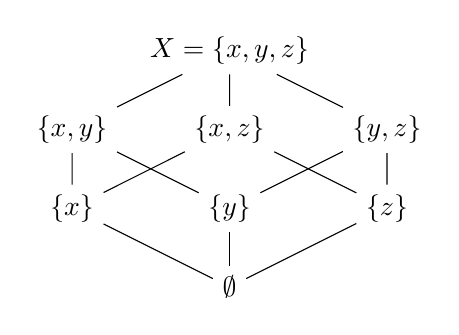
\begin{tikzpicture}
  \node (X)  at (2,3) {$X = \{x, y, z\}$};
  \node (xy) at (0,2) {$\{x, y\}$};
  \node (xz) at (2,2) {$\{x, z\}$};
  \node (yz) at (4,2) {$\{y, z\}$};
  \node (x)  at (0,1) {$\{x\}$};
  \node (y)  at (2,1) {$\{y\}$};
  \node (z)  at (4,1) {$\{z\}$};
  \node (0)  at (2,0) {$\emptyset$};
  \draw(X)--(xy)--(x)--(0)--(z)--(yz)--(X);
  \draw(X)--(xz)--(x);
  \draw(xy)--(y)--(yz);
  \draw(z)--(xz);
  \draw(0)--(y);
\end{tikzpicture}
\caption{問\ref{renshu:bounds}のハッセ図}
\label{fig:hasse} 
\end{figure}

\begin{renshu}{}{}
\begin{enumerate}
  \item 正の整数$x, y \in \bbN^+$において,「$x$は$y$を割り切る」という関係を$x \preceq y$と表す.
  任意の正整数$a,b$をとってきたとき,その最大元/最小限,上界/下界,上限/下限はそれぞれなんだろうか.
  % 最大限:存在しない 上界:公倍数 上限:最小公倍数
  \item $\langle \mcalP(X), \subset \rangle$において,$A, B \subset X$の上界/下界,上限/下限はそれぞれなんだろうか.
  \item $X$を地球上に存在した/しているあらゆる生物の集合とし,$x, y \in X$に対して$x \preceq y$で「$x$は$y$の祖先か同一個体である」という関係を表す.ここから形成される半順序は生物系統樹と呼ばれる.この系統樹内のある部分集合$A \subset X$をとってきたとき,この生物集合は有界か,また上限・下限を持つか.
\end{enumerate}
\end{renshu}


\begin{rei}{}{}
順序集合の有界性についての問題は,哲学で非常によく出くわす.
例えば神の宇宙論的証明や存在論的証明の議論を順序の概念を用いてモデル化するとどうなるだろうか.

参考(神の宇宙論的証明):存在するあらゆるものは,原因を持つ.しかし時空間は有限であるので,因果の系列は無限に遡ることはできない.よって「原因をもたない原因」ないし「不動の第一動者(アリストテレス)」としての神が存在する.これは因果順序における最小元の存在の主張だ.ではそれはどのような証明だろうか.
\end{rei}


\section{単調写像}
我々は集合のところで,異なる集合$X, Y$間を「橋渡し」するものとしての関数$f:X \to Y$を見た.
同様に,二つの順序$\langle X, \preceq_X \rangle$, $\langle Y, \preceq_Y \rangle$が与えられたとき,前者を後者にマップさせることを考えたい.
ただしここで,$\preceq_X, \preceq_Y$はそれぞれ集合$X,Y$上に定義された前/半/全順序関係である.

二つの順序の対応として,もととなっている集合$X, Y$の間の関数$f:X \to Y$を考える.
しかしこの関数が$X$の順序をめちゃくちゃにしてしまったら,「順序の対応」とはいえない.
むしろ$X$の大小関係が,$Y$においてもしっかりと保たれていてほしい.
これを数学的には,順序の\emph{構造を保つ写像}(structure-preserving map)という.
それは具体的には次で与えられる:
\begin{dfn}{単調写像}{}
関数$f:X \to Y$が次の条件を満たすとき,順序$\langle X, \preceq_X \rangle$, $\langle Y, \preceq_Y \rangle$の間の\emph{単調写像}(monotone map)といわれる
\[
 \text{すべての}x, x' \in X \text{に対して, }  x \preceq_X x' \text{ ならば } f(x) \preceq_Y f(x').
\]
\end{dfn}
つまり$x$より$x'$のほうが大きいなら,それぞれを$Y$に飛ばした$f(x)$より$f(x')$のほうが大きくなっている,ということだ.
ここで,左辺は$X$上の順序$\preceq_X$であるのに対し,右辺は$Y$上の順序$\preceq_Y$で比較されていることに注意.
よって上の条件は,$\preceq_X$で定めれられる$X$の順序構造が,$Y$において$\preceq_Y$として保たれている,ということを定めている.

\begin{rei}{}{}
 \begin{enumerate}
  \item 整数$\bbN$を実数$\bbR$に埋め込む関数$f:x \mapsto x$を考えると,これは当然$\langle \bbN, \leq \rangle$, $\langle \bbR, \leq \rangle$の間の単調写像になっている.
  \item 整数を2倍する関数$f:x \mapsto 2x$は,$\langle \bbN, \leq \rangle$とそれ自身の間の単調写像である.
  \item 素点(0〜100点)を評語(F, D, C, B, A, A+)に換算する成績評価関数は,単調写像である(でないと困る).
 \end{enumerate}
\end{rei}

以上はいずれも全順序間の写像であったが,半順序から全順序,のような単調写像も考えることができる.
例えば生命の分類体系(taxonomy)は,図\ref{fig:taxonomy}のような半順序をなす.
これをそれぞれの分類階級(種,属,科・・・)に対応させる関数を考えると,これは半順序から全順序への単調写像になっている.
\begin{figure}[h]
\centering
\begin{tikzpicture}
  \node (sp) at (0,4.5) {サピエンス};
  \node (hb) at (2,4.5) {ハビリス};
  \node (ln) at (4,4.5) {ライオン};
  \node (tg) at (6,4.5) {トラ};
  \node (hm) at (2,3) {ホモ};
  \node (ct) at (4,3) {ネコ};
  \node (pr) at (2,1.5) {霊長};
  \node (cr) at (4,1.5) {食肉};
  \node (mm) at (3,0) {哺乳};
  \draw[<-](mm)--(pr);
  \draw[<-](pr)--(hm);
  \draw[<-](hm)--(sp);
  \draw[<-](hm)--(hb);
  \draw[<-](mm)--(cr);
  \draw[<-](cr)--(ct);
  \draw[<-](ct)--(ln);
  \draw[<-](ct)--(tg);

  \node (or) at (10,0) {目};
  \node (fa) at (10,1.5) {科};
  \node (ge) at (10,3) {属};
  \node (sc) at (10,4.5) {種};
  \draw[->](sc)--(ge);
  \draw[->](ge)--(fa);
  \draw[->](fa)--(or);

  \draw[->, dashed] (sp) to [out=20, in=160] (sc);
  \draw[->, dashed] (hb) to [out=15, in=165] (sc);
  \draw[->, dashed] (ln) to [out=10, in=170] (sc);
  \draw[->, dashed] (tg) to [out=5, in=175] (sc);

  \draw[->, dashed] (hm) to [out=15, in=165] (ge);
  \draw[->, dashed] (ct) to [out=10, in=170] (ge);

  \draw[->, dashed] (pr) to [out=15, in=165] (fa);
  \draw[->, dashed] (cr) to [out=10, in=170] (fa);

  \draw[->, dashed] (mm) to [out=10, in=170] (or);
\end{tikzpicture}
\caption{分類体系の単調写像(この例はFong \& Spivak, 『活躍する圏論』, p. 18より拝借した)}
\label{fig:taxonomy} 
\end{figure}
単調写像とは,このように二つの順序を横に並べて描いたとき,写像の対応を示す線(図\ref{fig:taxonomy}の点線矢印)が互いにクロスしない,という条件だと理解できる.

\begin{rei}{真理値関数}{truthvalue}
事例\ref{rei:logic} の論理式間の証明関係の前順序$\langle L, \vdash \rangle$を思い出そう.
それとは別に$\bbB = \{ \texttt{false}, \texttt{true} \}$からなる二元集合上に全順序$\texttt{false} \leq \texttt{true}$を導入する.
論理式への真理値割当を関数$f:L \to \bbB$によって表すとすると,この関数はどのようなものでなければならないか.
\end{rei}

\begin{rei}{測定理論}{ordinal}
$\langle X, \preceq \rangle$をなんらかの物の集合$X$の間の何らかの全順序であるとする.
実数値関数$\phi:X \to \bbR$が$\langle X, \preceq \rangle$と$\langle \bbR, \leq \rangle$の間の単調写像であるとき,$\phi$を\emph{順序尺度}(ordinal scale)という.

順序尺度は,物事の数値測定のうち最も単純なもので,$x_1, x_2, \dots$の順番を数値$\phi(x_1), \phi(x_2), \dots$で表す.
このとき,数値間の大小は$X$の間の順序を反映しているが,その間隔や比率などには意味がない.
なので数値を足したりかけたりすることはできない.
これは,ここで使われている道具立てが単に順序集合に過ぎず,足し算や掛け算などの演算を備えていない,という事実を反映している.
\end{rei}

\begin{renshu}{}{}
 順序尺度の例をあげ,それが単調性を満たしていることを確認せよ.
\end{renshu}

単調写像は極めて単純な道具立てに思える(単に順序を別の順序にうつしているだけじゃないか!).
しかしここにはすでに,複数の重要な哲学的含意がある.

まず事例\ref{rei:truthvalue}は,意味論的な含意を示す.
意味論とは,統語的表現とその意味,あるいはその真偽値の間の関係である.
我々はその間に,なんらかの法則的関係が成り立っていることを期待する.
この事例では,命題論理の証明関係と,その真偽値の間の関係性が,単調写像によって捉えられていることに注意しよう.

次に事例\ref{rei:ordinal}は,認識論的な含意を示す.
というのも測定理論とは,形式化された認識論だからである.
それは,ある事物の体系(世界)を,数的表現の体系(記述)へと写し取ることを目指している.
その際,我々の記述は世界の構造を写し取ったものであってほしい.
順序というのはそうした構造のうちの,単純ではあるが重要なものの一つであり,単調性はその構造が数の構造へとしっかりと写し取られている,ということを保証するものである.
つまり大げさにいえば,構造を保つ写像は認識の正しさを保証しているのである(こうした見方は,例えばウィトゲンシュタインの\emph{言語の写像理論}(Picture theory of language)に強く現れている).

我々は今後,様々な数学的構造を見ていくが,その都度,その構造を保存する写像が何かを考えていく(数学的にはこれは\emph{準同型写像}(homomorphism)ともいわれる).
ある構造から別の構造への準同型写像を,数学では\emph{表現}(representation),またそうした表現が存在することを証明する定理を\emph{表現定理}という.
表現は非常に重要な概念であり,数学の至る所に出てくるし,また「表現論」という分野の名前にもなっている\footnote{表現論は,群のところで触れるが,群から線形写像(行列)への群準同型写像を考える.}.
上の事例は,それぞれ証明帰結関係の真理値による表現,事物の大小関係の数値による表現,ということができる.


\begin{renshu}{単調写像の合成}{}
$\langle X, \preceq_X \rangle, \langle Y, \preceq_Y \rangle, \langle Z, \preceq_Z \rangle$を前順序とする.
$f:X \to Y, g:Y \to Z$が単調写像ならば,その合成$g \circ f: X \to Z$も単調写像になることを示せ. 
\end{renshu}


\section{同型写像}
単調写像は$\langle X, \preceq_X \rangle$から$\langle Y, \preceq_Y \rangle$への一方向的な関係であった.
次はこれを双方向的に考えてみよう.
上の練習問題で単調写像の合成性を見たが,ここで$Z$を$X$にして$X \xrightarrow{f} Y \xrightarrow{g} X$と戻ってくるようにすると合成$g \circ f$は$X$から$X$への単調写像である.
同型とは,このような合成写像によって任意の$x \in X$に対してもとの場所$x$に帰ってくることができることをいう.

\begin{dfn}{同型写像}{}
$\langle X, \preceq_X \rangle, \langle Y, \preceq_Y \rangle$を前順序とする.
単調写像$f:X \to Y$に対し,任意の$x \in X, y \in Y$に対し,
\[
 x = g(f(x)) \ \ \ \ \ \ y = f(g(y))
\]
を満たすような「帰りの」単調写像$g:Y \to X$があるとき,$f$を\emph{同型写像}(isomorphism)と呼ぶ.
また同型写像$X \to Y$が存在するとき,前順序$X$と$Y$は\emph{同型}(isomorphic)であるという.
\end{dfn}
言い換えれば,同型写像とは全単射(前章7節)であるような単調写像,ということにほかならない.

同型であるような順序集合は,基本的には集合の中身が違うだけで,順序としては全く同一である.
つまり図\ref{fig:hasse}のようなハッセ図で表すと,ノードのラベルが違うだけで,図の形としては全く同じになる.


\begin{rei}{心身並行論}{parallelism}
因果関係「$x$は$y$の原因である」が前順序を構成するとしよう(便宜的に,すべてのものはそれ自身の原因でもあると考える).
$\langle P, \to_P \rangle, \langle M, \to_M \rangle$をそれぞれ,物的対象$P$および心的対象$M$の間の因果的順序であるとする.
\emph{心身並行論}(cf. スピノザ)とは,二つの前順序$P, M$が同型であるという主張だと解釈できる.
\end{rei}

\begin{hatten}{}{}
心身並行論からは,すべての物的事象は固有の心的対応物を持つこと,すなわち汎心論が帰結する.
汎心論を避ける形で,しかし心的事象の間の因果関係を物的事象の間の因果関係に基づけるためには,どうすればよいだろうか.
\end{hatten}

最後に少し進んだ話題を一つ.
同型写像は行って戻ってきたときにちょうど元のところに帰る,という意味でなかなかに強い条件である.
これを緩めて,行って戻ったきたら元の要素より必ず大きくなっている,つまり任意の$x \in X, y \in Y$に対し
\[
 x \preceq_X g(f(x)) \ \ \ \ \ \ y \preceq_Y f(g(y))
\]
という条件を考えることもできる.
こうした単調写像の対$f:X \to Y, g:Y \to X$は,\emph{ガロア接続}(Galois connection)と呼ばれる.



\end{document}
